\chapter{Ich bin ein Kapitel}
\label{sec:regelung}

%----------------------------------------------------------------------------------------------
\section{Ich bin ein Titel}
\label{sec:ichbineintitel}
%----------------------------------------------------------------------------------------------

Dumm ist der der dummes tut. Dumm ist der der dummes tut. Dumm ist der der dummes tut. Dumm ist der der dummes tut. Dumm ist der der dummes tut. Dumm ist der der dummes tut. Dumm ist der der dummes tut. Dumm ist der der dummes tut. Dumm ist der der dummes tut.\\ % \\ --> Neue Zeile
Dumm ist der der dummes tut. Dumm ist der der dummes tut. Dumm ist der der dummes tut. Dumm ist der der dummes tut. Dumm ist der der dummes tut. Dumm ist der der dummes tut. Dumm ist der der dummes tut. Dumm ist der der dummes tut. Dumm ist der der dummes tut.
% Abstand --> Neuer Absatz

Dumm ist der der dummes tut. Dumm ist der der dummes tut. Dumm ist der der dummes tut. Dumm ist der der dummes tut. Dumm ist der der dummes tut. Dumm ist der der dummes tut. Dumm ist der der dummes tut. Dumm ist der der dummes tut. Dumm ist der der dummes tut.

\subsection{Ich bin ein Untertitel}

Dumm ist der der dummes tut. Dumm ist der der dummes tut. Dumm ist der der dummes tut. Dumm ist der der dummes tut. Dumm ist der der dummes tut. Dumm ist der der dummes tut. Dumm ist der der dummes tut. Dumm ist der der dummes tut. Dumm ist der der dummes tut. 

\subsubsection{Ich bin ein Unter-Untertitel}

Dumm ist der der dummes tut. Dumm ist der der dummes tut. Dumm ist der der dummes tut. Dumm ist der der dummes tut. Dumm ist der der dummes tut. Dumm ist der der dummes tut. Dumm ist der der dummes tut. Dumm ist der der dummes tut. Dumm ist der der dummes tut. 

\minisec{Ich bin ein Unter-Untertitel mit wenig Abstand bis zum Text}

Dumm ist der der dummes tut. Dumm ist der der dummes tut. Dumm ist der der dummes tut. Dumm ist der der dummes tut. Dumm ist der der dummes tut. Dumm ist der der dummes tut. Dumm ist der der dummes tut. Dumm ist der der dummes tut. Dumm ist der der dummes tut. 

\newpage % -> Begine auf einer neuen Seite
%----------------------------------------------------------------------------------------------
\section{Einige Gleichungen}
%----------------------------------------------------------------------------------------------

\subsection{Eine Gleichung}

\eq{
	y = f\left(x\right)
}

\subsection{Eine Gleichungsfolge mit Text}

% Befehl von pmic \seq
\seq{
 	u &= R_1i_1 + L_1\frac{d}{dt}i_1 -M\frac{d}{dt}i_2 + k_{m1}\frac{d}{dt}x & \mbox{(Spule bzw. Spulenpaar)} \label{eq:voice_coil_dynamik_a}\\
 	0 &= R_2i_2 + L_2\frac{d}{dt}i_2 -M\frac{d}{dt}i_1 + k_{m2}\frac{d}{dt}x & \mbox{(Kurzschlussring)}\\
 	m\frac{d^2}{dt^2}x &= w_{e1}i_1 + w_{e2}i_2 & \mbox{(Mechanik)}
	\label{eq:voice_coil_dynamik_c}
}

\subsection{Matrizen}

\minisec{Zwei Matrizen}

\begin{align}
\mh{A}_{ds} &= 
	\left[
		\begin{array}{rrrrrr}
    0.8565  &  0.0218  &  0.0211  & -0.0096  & -0.0050  &  0.0080 \\
    0.0156  &  0.8659  &  0.0222  &  0.0019  &  0.0226  &  0.0124 \\
    0.0154  &  0.0204  &  0.8655  &  0.0034  & -0.0070  & -0.0080 \\
   -0.0003  & -0.0041  &  0.0042  &  0.9444  &  0.0051  &  0.0039 \\
    0.0043  & -0.0018  & -0.0037  &  0.0062  &  0.9452  &  0.0066 \\
   -0.0040  &  0.0034  &  0.0004  &  0.0034  &  0.0058  &  0.9447
		\end{array}
	\right] \notag \\
	\mh{B}_{ds} &= 
	\left[
		\begin{array}{rrrrrr}
   23.6438  & -4.1978  & -4.5305  & -1.0673  & -0.6754  &  2.8364 \\
    1.5117  & 20.5480  & -4.9742  &  0.5737  &  4.3086  &  1.1824 \\
   -3.5779  & -2.1936  & 21.4407  & -0.4329  &  0.6942  & -0.9001 \\
    0.1868  &  0.7024  & -1.0351  & 12.8674  & -3.3410  & -1.6403 \\
   -1.0520  &  0.2974  &  0.7386  &  1.5430  & 14.8812  & -3.2842 \\
    0.8054  & -0.7401  & -0.0076  & -1.5063  & -0.0413  & 14.7114
	  \end{array}
	\right] 
\end{align}

\minisec{Eine etwas speziellere Matrix}

\begin{align}
	\frac{\partial \m{q}_i(\m{x})}{\partial \m{x}}\bigg|_{\m{x}_0} = \m{J}_i(\m{x}_0) := 
	\left[
		\begin{array}{cccc} 
			\displaystyle\frac{\partial q_{i1}(x_0)}{\partial x} & \displaystyle\frac{\partial q_{i1}(y_0)}{\partial y} & \ldots & \displaystyle\frac{\partial q_{i1}(\varphi_{z0})}{\partial \varphi_z} \\
			\displaystyle\frac{\partial q_{i2}(x_0)}{\partial x} & \displaystyle\frac{\partial q_{i2}(y_0)}{\partial y} & \ldots & \displaystyle\frac{\partial q_{i2}(\varphi_{z0})}{\partial \varphi_z} \\
			\vdots&\vdots&\ddots&\vdots\\
			\displaystyle\frac{\partial q_{i6}(x_0)}{\partial x} & \displaystyle\frac{\partial q_{i6}(y_0)}{\partial y} & \ldots & \displaystyle\frac{\partial q_{i6}(\varphi_{z0})}{\partial \varphi_z} \\
		\end{array}	
	\right]
	\label{eq:jacobi_vt}
\end{align}

%----------------------------------------------------------------------------------------------
\section{Tabellen}
%----------------------------------------------------------------------------------------------

\begin{table}[H]
	\centering
	\captionabove{Modellparameter bei einer Spule}
		\begin{tabular}{|ccccc|}
			\hline
			\rowcolor{Gray}
			$R_1 [\Omega]$ & $R_2 [\mbox{m}\Omega]$ & $L_1 [\mbox{mH}]$ & $L_2 [\mbox{mH}]$ & $M [\mbox{mH}]$ \\
			\hline
			\hline
			$607.0$ & $0.1$ & $60.37$ & $1.90\cdot10^{-5}$ & $ 2.83\cdot10^{-2}$\\
			\hline
		\end{tabular}
		\label{tab:identifizierte_modellparameter_1_spule}
		\vspace{0.4cm}
		\captionabove{Modellparameter bei Parallelschaltung von zwei Spulen}
		\begin{tabular}{|ccccc|}
			\hline
			\rowcolor{Gray}
			$R_1 [\Omega]$ & $R_2 [\mbox{m}\Omega]$ & $L_1 [\mbox{mH}]$ & $L_2 [\mbox{mH}]$ & $M [\mbox{mH}]$ \\
			\hline
			\hline
			$304.0$ & $0.1$ & $57.85$ & $2.20\cdot10^{-5}$ & $3.00\cdot10^{-2}$\\
			\hline
		\end{tabular}
		\label{tab:identifizierte_modellparameter_2_spulen_parallel}
\end{table}

%----------------------------------------------------------------------------------------------
\section{Grafiken}
%----------------------------------------------------------------------------------------------

\subsection{Normale Grafik}

Hier eine normale Grafik.

\begin{figure}[ht]
	\centering
		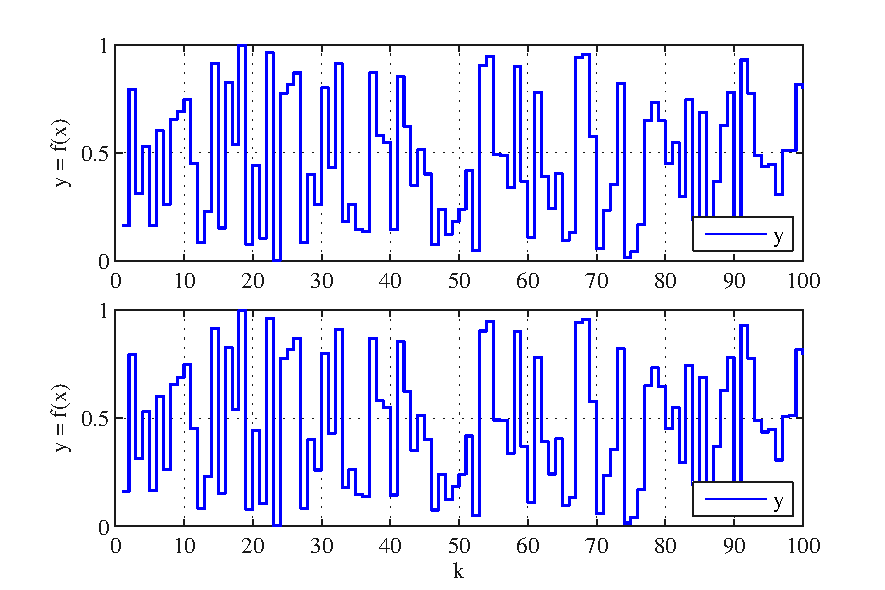
\includegraphics{images/grafik2.pdf}
	\caption{Hier steht etwas �ber die Grafik}
	\label{fig:grafik2}
\end{figure}

Hier ein Bode-Diagramm.

\begin{figure}[H]
	\centering
		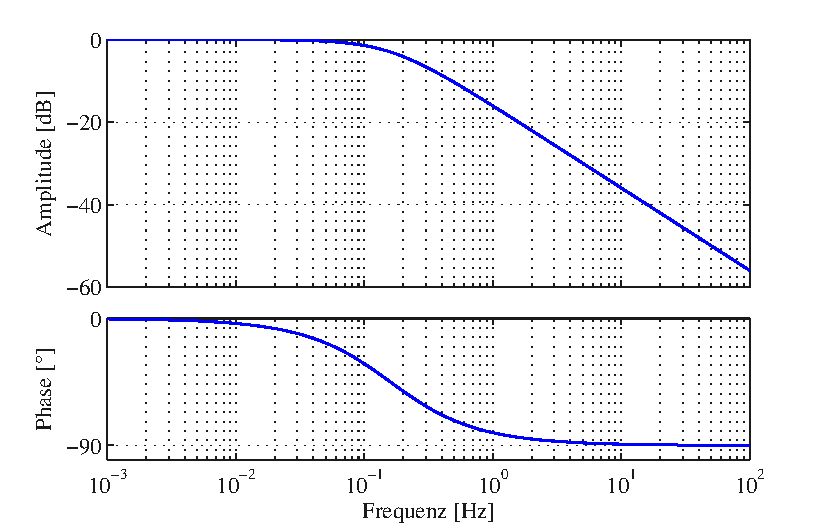
\includegraphics{images/grafik3.pdf}
	\caption{Hier steht etwas �ber die Grafik}
	\label{fig:grafik3}
\end{figure}

\subsection{Mehrere Grafiken nebeneinander}

\begin{figure}[ht]
\centering
		\subfloat[Hier k�nnen auch Formeln stehen $\m{G}(j\omega)$]{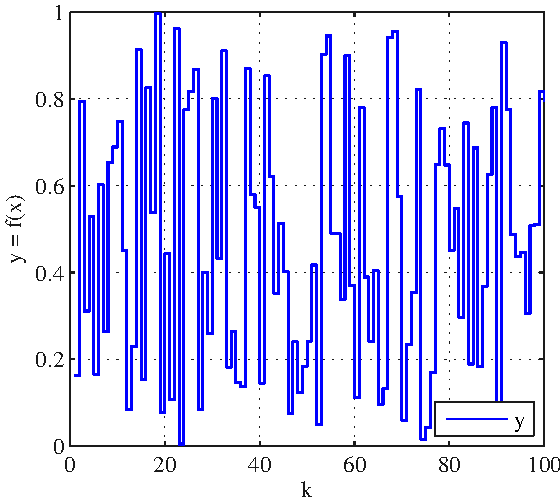
\includegraphics[width=0.50\textwidth]{images/grafik1.pdf}}
		\subfloat[Und auch hier $\m{G}(j\omega)$]{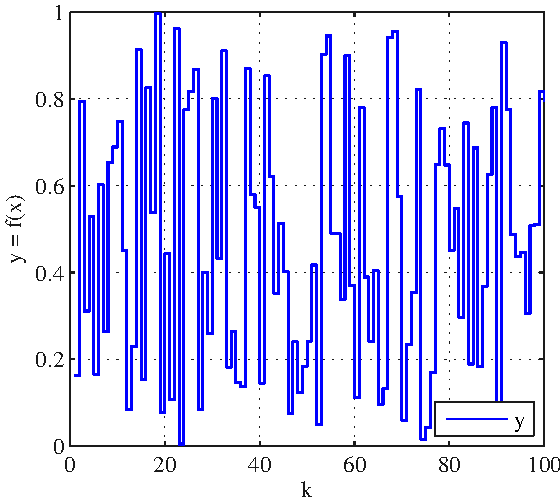
\includegraphics[width=0.50\textwidth]{images/grafik1.pdf}}
	\caption{Hier steht etwas �ber die Grafik}
	\label{fig:grafik12}
\end{figure}

\subsection{Grafik neben Text mit der Umgebung Minipage}

\begin{figure}[H]
	\begin{minipage}[b]{0.5\textwidth} 
		Dumm ist der der dummes tut. Dumm ist der der dummes tut. Dumm ist der der dummes tut. Dumm ist der der dummes tut. Dumm ist der der dummes tut. Dumm ist der der dummes tut. Dumm ist der der dummes tut. Dumm ist der der dummes tut. Dumm ist der der dummes tut.
		\vspace{4.1cm}
	\end{minipage}
	\begin{minipage}[b]{0.5\textwidth}
		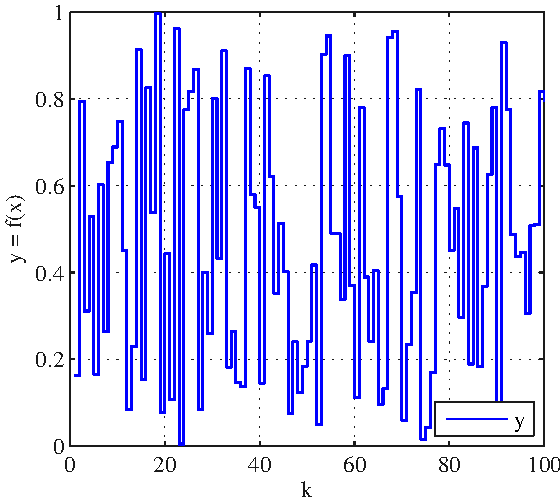
\includegraphics[width=1\textwidth]{images/grafik1.pdf}
	\end{minipage}
\end{figure}

\subsection{Eine Grafik aus Inkscape}

\begin{figure}[H]
	\centering
	\def\svgwidth{15cm}
		\input{images/skalierung_mimo_blockschaltbild.pdf_tex}
	\caption{Hier steht etwas �ber die Grafik}
	\label{fig:skalierung_mimo_blockschaltbild}
\end{figure}

%----------------------------------------------------------------------------------------------
\section{Verweise, Literaturangaben}
%----------------------------------------------------------------------------------------------

Ich bin ein Literaturverweis \cite{altb1}. Ich bin sogar zwei Literaturverweise \cite{lunze1,lunze2}.

Ich bin eine Referenz auf die Abbildung \ref{fig:skalierung_mimo_blockschaltbild}.

Ich bin eine Referenz auf das Kapitel \ref{sec:ichbineintitel}.